\documentclass[18pt, compress, aspectratio=169]{beamer}

% can be compiled by xelatex -shell-escape presentation.tex

\usetheme[]{m}

\usepackage[utf8]{inputenc}
\usepackage[russian, english]{babel}
\usepackage{booktabs}
\usepackage[scale=2]{ccicons}
\usepackage{listings}
\usepackage{marvosym}
\usepackage{color}
\usepackage{xcolor}
\usepackage[document]{ragged2e}
\usepackage[export]{adjustbox}
\usepackage{fontawesome}
\usepackage{enumitem}
\usepackage{minted}
\usemintedstyle{tango}
\usepackage[normalem]{ulem}
%\usemintedstyle{monokai}

\usetikzlibrary{shapes,arrows,positioning}
\graphicspath{{images/}}
\newfontfamily{\FA}{FontAwesome}

\definecolor{check}{rgb}{0.1,2,0.3}
\definecolor{fail}{rgb}{2,0.1,0.1}
\definecolor{question}{rgb}{0.9,0.9,0.0}

\def\twitter{{\FA \faTwitter}}
\def\github{{\FA \faGithubSign}}
\def\email{{\FA \faEnvelope}}
\def\check{\textcolor{check}{\FA \faCheck}}
\def\fail{\textcolor{fail}{\FA \faRemove}}
\def\question{\textcolor{question}{\FA \faSearch}}

\renewcommand{\ttdefault}{pcr}
\newfontfamily{\ttfamily}{Fira Code}
\makeatletter
\newcommand\HUGE{\@setfontsize\Huge{32}{41}}
\makeatother

\renewcommand{\ULthickness}{2.0pt}

\definecolor{links}{HTML}{0099FF}
\hypersetup{colorlinks, linkcolor=, urlcolor=links}

\setbeamerfont{section title}{family=\Book, size=\Huge, shape=\normalfont}
\setbeamerfont{frametitle}{family=\Book, size=\large, shape=\normalfont}
\setbeamerfont{title}{family=\Book, size=\HUGE, shape=\normalfont}
\setbeamerfont{subtitle}{size=\LARGE}
\usebackgroundtemplate{
\includegraphics[width=\paperwidth]{slide_background.jpg}}

\setbeamertemplate{title page}
{
  \begin{minipage}[b][\paperheight]{\textwidth}
    \vspace*{3em}

    \ifx\inserttitle\@empty\else
    {{% \inserttitle is nonempty
      \raggedright%
      \linespread{1.0}%
      \usebeamerfont{title}%
      \usebeamercolor[fg]{title}%
      \if@noSmallCapitals%
        \inserttitle%
      \else%
        \scshape\MakeLowercase{\inserttitle}%
      \fi%
      \vspace*{0.5em}
    }}
    \fi

    \ifx\insertsubtitle\@empty\else
    {{% \insertsubtitle is nonempty
      \usebeamerfont{subtitle}%
      \usebeamercolor[fg]{subtitle}%
      \insertsubtitle%
      \vspace*{0.5em}%
    }}
    \fi
    \vfill
    \vspace*{2em}
  \end{minipage}
}

\setbeamertemplate{section page}
{
  \vspace{2em}
  \centering
  \begin{minipage}{22em}
    \usebeamercolor[fg]{section title}
    \usebeamerfont{section title}
    \insertsectionHEAD\\[-1ex]
  \end{minipage}
  \par
}

\setbeamertemplate{footline}
{
\begin{beamercolorbox}[wd=\textwidth,ht=3ex,dp=3ex,leftskip=0.3cm,rightskip=0.3cm]{structure}
  \usebeamerfont{page number in head/foot}
  \insertframenumber
\end{beamercolorbox}
}

\title{NoSQL внутри SQL}
\subtitle{приземленные вопросы\\ практического применения}
\date{\today}
\institute{}

\begin{document}
{
  \usebackgroundtemplate{
\includegraphics[width=\paperwidth]{title_background.jpg}}%
  \fontsize{17pt}{18}\selectfont
  \maketitle
}

\fontsize{21pt}{23}\selectfont
\section{}

\begin{frame}{}
    \begin{itemize}[label={}]
        \item 
\includegraphics[scale=0.04]{mindojo_logo.png} Дмитрий Долгов, Mindojo
        \item {\github\ github.com/erthalion}
        \item {\twitter\ @erthalion}
        \item \email\ 9erthalion6 at gmail dot com
    \end{itemize}
\end{frame}

\begin{frame}[fragile]
    \frametitle{}
    \begin{center}
        \textbf{Данные}
    \end{center}
    \begin{itemize}[leftmargin=*]
        \item <+->
    \end{itemize}

    \vspace{-40pt}

    \begin{columns}[T,onlytextwidth]
    \column{0.5\textwidth}
    \begin{itemize}[leftmargin=*]
        \item <+->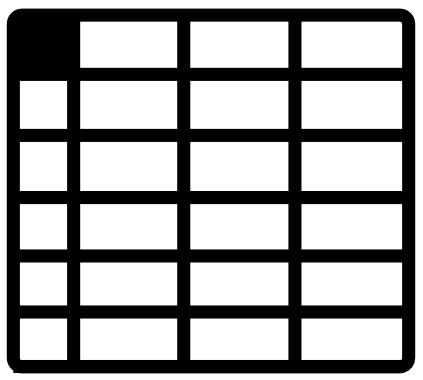
\includegraphics[width=6cm,height=5cm]{relation.png}
    \end{itemize}

    \vspace{20pt}

    \column{0.5\textwidth}
    \begin{itemize}[leftmargin=*]
        \item <+->
\includegraphics[width=6cm,height=5cm]{document.jpg}
    \end{itemize}
    \end{columns}
\end{frame}

\begin{frame}
    \frametitle{}
    \begin{center}
        \textbf{Данные нужно хранить в соответствующем формате:}
        \pause
        \begin{itemize}[label={\MVRightarrow}]
            \item <+-> Отдельные хранилища,\\ единый интерфейс
            \item <+-> Единое хранилище,\\ разные форматы
        \end{itemize}
    \end{center}
\end{frame}

\begin{frame}
    \frametitle{}
    \begin{center}
        \textbf{Отдельные хранилища}
        \pause
        \begin{itemize}[label={\MVRightarrow}]
            \item <+-> Конкретный формат обрабатывается наилучщим образом \check
            \item <+-> Производительность, дублирование \question
            \item <+-> Вопросы интеграции компонентов \fail
        \end{itemize}
    \end{center}
\end{frame}

\begin{frame}
    \frametitle{}
    \begin{center}
        \textbf{Единое хранилище}
        \pause
        \begin{itemize}[label={\MVRightarrow}]
            \item <+-> Не требует интеграции \check
            \item <+-> Производительность, дублирование \question
            \item <+-> Поддержка со стороны БД \question
        \end{itemize}
    \end{center}
\end{frame}
\note{
    если данные разного формата не сравнимы по объему, затраты на интеграцию
    и инфраструктуру могут не окупиться.
}

\begin{frame}
    \frametitle{}
    \begin{center}
    %\vspace{-10pt}
    \begin{figure}
        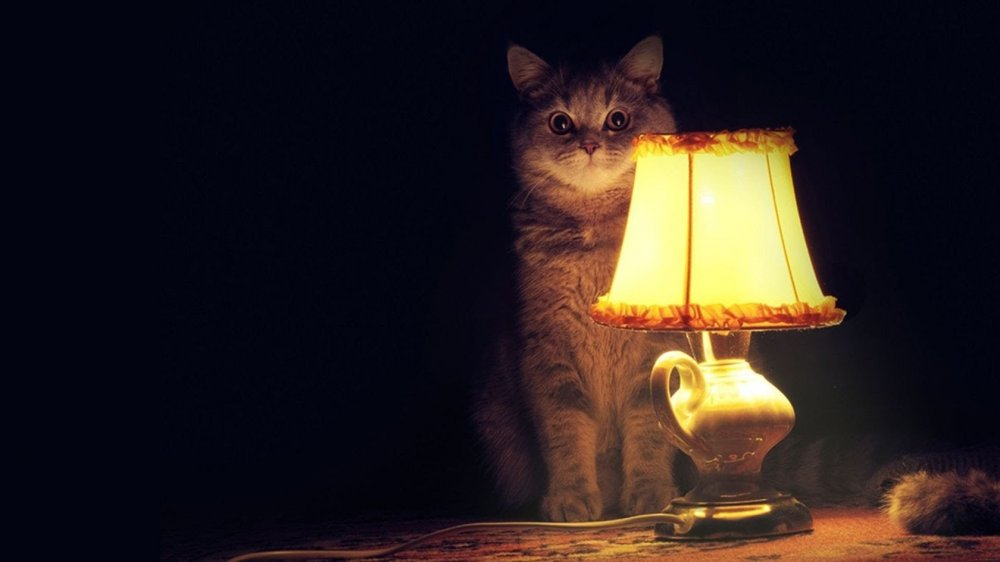
\includegraphics[width=0.9\textwidth,center]{cat_stories.jpg}
    \end{figure}
    \end{center}
\end{frame}

\begin{frame}
    \frametitle{}
    \begin{center}
        \textbf{Кто?}
        \begin{itemize}[label={\MVRightarrow}]
            \item Postgresql (hstore/json/jsonb)
            \item MySQL (json)
            \item Oracle
            \item MSSql
            \item db2
        \end{itemize}
    \end{center}
\end{frame}

\fontsize{13pt}{14}\selectfont
\begin{frame}
    \frametitle{}
    \vspace{2em}
    \centering
    \begin{minipage}{32em}
        \usebeamercolor[fg]{section title}
        \usebeamerfont{section title}
        Легкий способ начать \sout{бегать по утрам} использовать документы в реляционной базе
    \end{minipage}
\end{frame}
\fontsize{17pt}{18}\selectfont

\begin{frame}
    \frametitle{}
    \begin{center}
    \inputminted[
        fontsize=\Large,
    ]{sql}{sql/json_build.sql}
    \end{center}
\end{frame}

\begin{frame}
    \frametitle{}
    \begin{center}
    \inputminted[
        fontsize=\Large,
    ]{sql}{sql/json_agg.sql}
    \end{center}
\end{frame}

\begin{frame}
    \frametitle{}
    \begin{center}
    \inputminted[
        fontsize=\Large,
    ]{sql}{sql/load.sql}
    \end{center}
\end{frame}

\begin{frame}
    \frametitle{}
    \begin{center}
        \begin{itemize}[label={\MVRightarrow}]
            \item Загрузка дампа из внешних источников
            \item Некорректные данные с валидной структурой - json5
            \item Битые данные - ручное исправление, линтеры
        \end{itemize}
    \end{center}
\end{frame}

\fontsize{13pt}{14}\selectfont
\section{Производительность}
\fontsize{17pt}{18}\selectfont

\begin{frame}
    \frametitle{}
    \begin{center}
        \textbf{Факторы}
        \pause
        \begin{itemize}[label={\MVRightarrow}]
            \item <+-> Структура данных на диске
            \item <+-> Сериализация данных
            \item <+-> Поддержка индексов
        \end{itemize}
    \end{center}
\end{frame}
\note{
    оптимизация по размеру и пробеганию
}

\begin{frame}
    \frametitle{}
    \begin{center}
    \textbf{Bson}
    \begin{figure}
        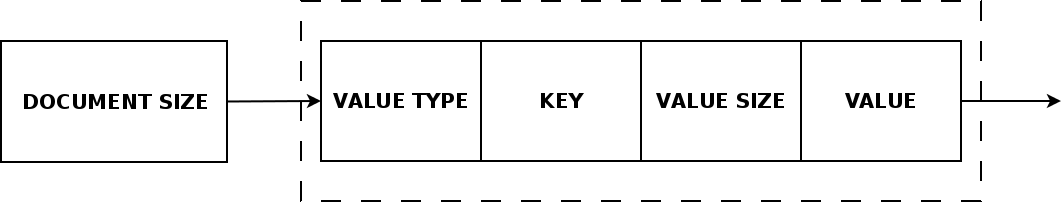
\includegraphics[width=1.0\textwidth,center]{bson.png}
    \end{figure}
    \end{center}
\end{frame}

\begin{frame}
    \frametitle{}
    \begin{center}
    \inputminted[
        fontsize=\Large,
    ]{python}{sql/bson.py}

    \begin{figure}
        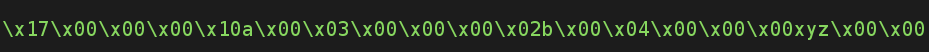
\includegraphics[width=1.0\textwidth,center]{bson_binary.png}
    \end{figure}

    \end{center}
\end{frame}

\begin{frame}
    \frametitle{}
    \begin{center}
    \textbf{Jsonb}
    \begin{figure}
        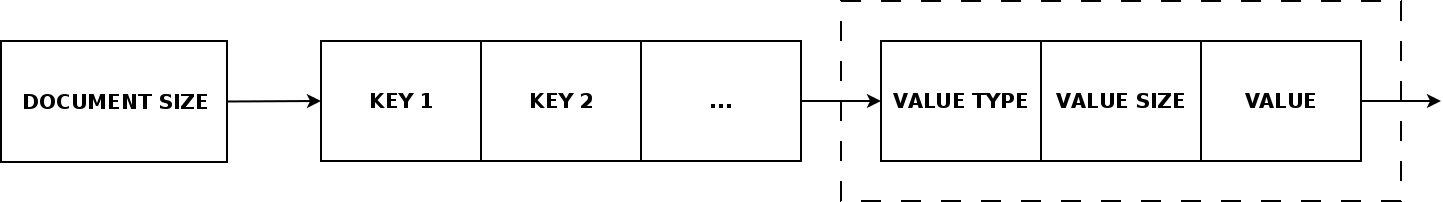
\includegraphics[width=1.0\textwidth,center]{jsonb.png}
    \end{figure}
    \end{center}
\end{frame}

\begin{frame}
    \frametitle{}
    \begin{center}
    \inputminted[
        fontsize=\Large,
    ]{python}{sql/jsonb_binary.sql}

    \begin{figure}
        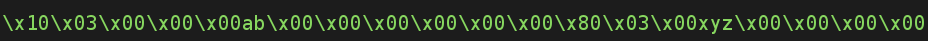
\includegraphics[width=1.0\textwidth,center]{jsonb_binary.png}
    \end{figure}

    \end{center}
\end{frame}

\begin{frame}
    \frametitle{}
    \begin{center}
    \textbf{MySQL json}
    \begin{figure}
        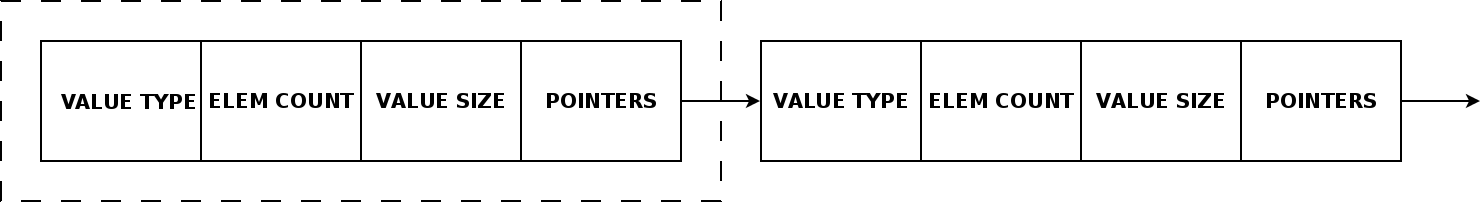
\includegraphics[width=1.0\textwidth,center]{mysql_json.png}
    \end{figure}
    \end{center}
\end{frame}

\begin{frame}
    \frametitle{}
    \textbf{Сериализация данных}
    \begin{center}
        \begin{itemize}[label={\MVRightarrow}]
            \item MongoDB - дерево Document -> Elements
            \item Postgresql - JsonbValue со списком элементов
            \item MySQL - ленивая структура с указателями
        \end{itemize}
    \end{center}
\end{frame}

\begin{frame}
    \frametitle{}
    \textbf{Индексы}
    \begin{center}
        \begin{itemize}[label={\MVRightarrow}]
            \item MongoDB - индексы для полей
            \item Postgresql - общий индекс, индексы для полей
            \item MySQL - виртуальные колонки для индексирования
        \end{itemize}
    \end{center}
\end{frame}

\fontsize{13pt}{14}\selectfont
\section{Тестирование}
\fontsize{17pt}{18}\selectfont

\begin{frame}
    \frametitle{}
    \begin{center}
    %\vspace{-10pt}
    \begin{figure}
        
\includegraphics[width=0.8\textwidth,center]{great_performance.jpg}
    \end{figure}
    \end{center}
\end{frame}

\begin{frame}
    \frametitle{}
    \begin{center}
        \begin{itemize}[label={}]
            \item YCSB 0.8, $10^{6}$
            \item 16GB memory, 4 core 2.3GHz
            \item Postgresql 9.5.4
            \item MongoDB 3.2.9
            \item MySQL 5.7.9
            \item AWS EC2 m4.xlarge
            \item 16GB memory, 4 core 2.3GHz
        \end{itemize}
    \end{center}
\end{frame}

\begin{frame}
    \frametitle{}
    \begin{center}
        \textbf{Воспроизводимость}
        \begin{itemize}[label={}]
            \item \href{https://github.com/erthalion/YCSB}{erthalion/YCSB}
            \item \href{https://github.com/erthalion/ansible-ycsb}{erthalion/ansible-ycsb}
        \end{itemize}
    \end{center}
\end{frame}

\begin{frame}
    \frametitle{}
    \begin{center}
        \textbf{Простая выборка по ключу с Btree индексом}
        \begin{itemize}[label={}]
            \item "Маленький документ"
            \item 10 полей
            \item без вложенности
        \end{itemize}
    \end{center}
\end{frame}

\begin{frame}
    \frametitle{}
    \begin{center}
    %\vspace{-10pt}
    \begin{figure}
        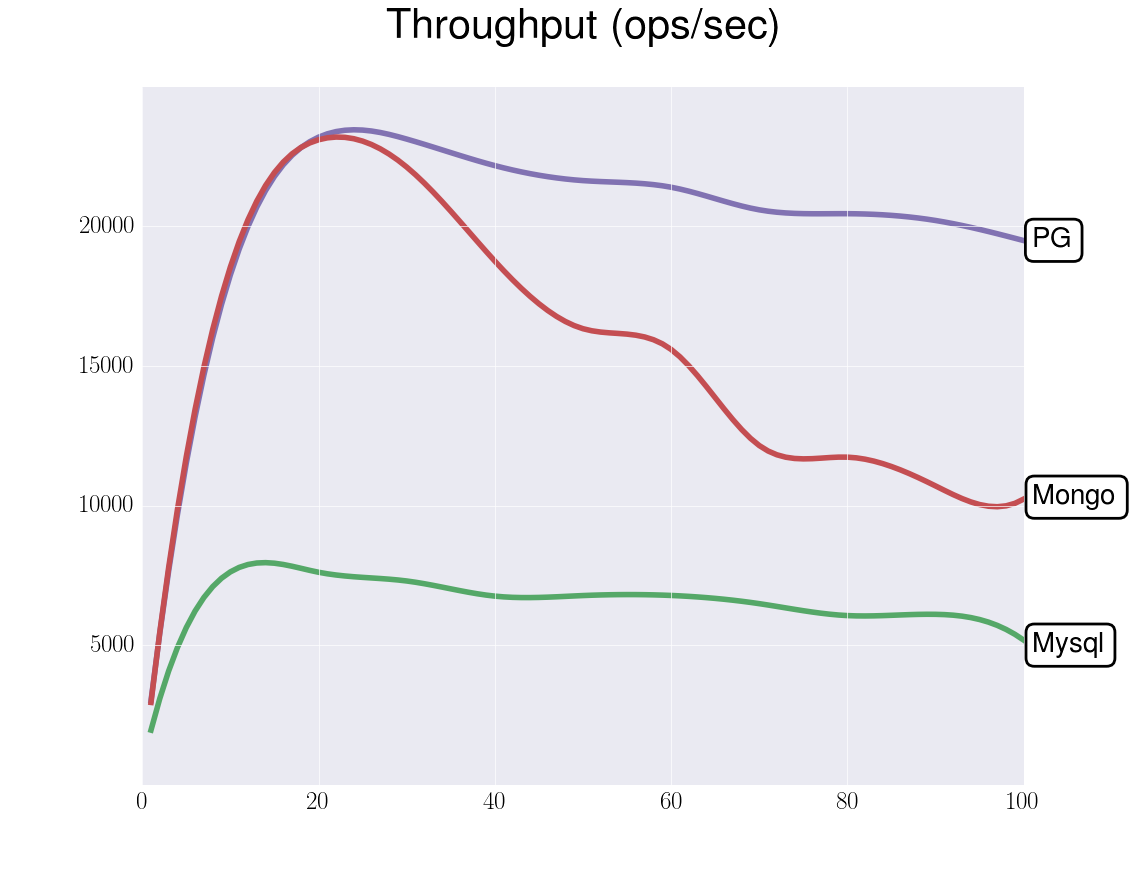
\includegraphics[width=0.75\textwidth,center]{benchmarks/simple_select_throughput.png}
    \end{figure}
    \end{center}
\end{frame}

\begin{frame}
    \frametitle{}
    \begin{center}
    %\vspace{-10pt}
    \begin{figure}
        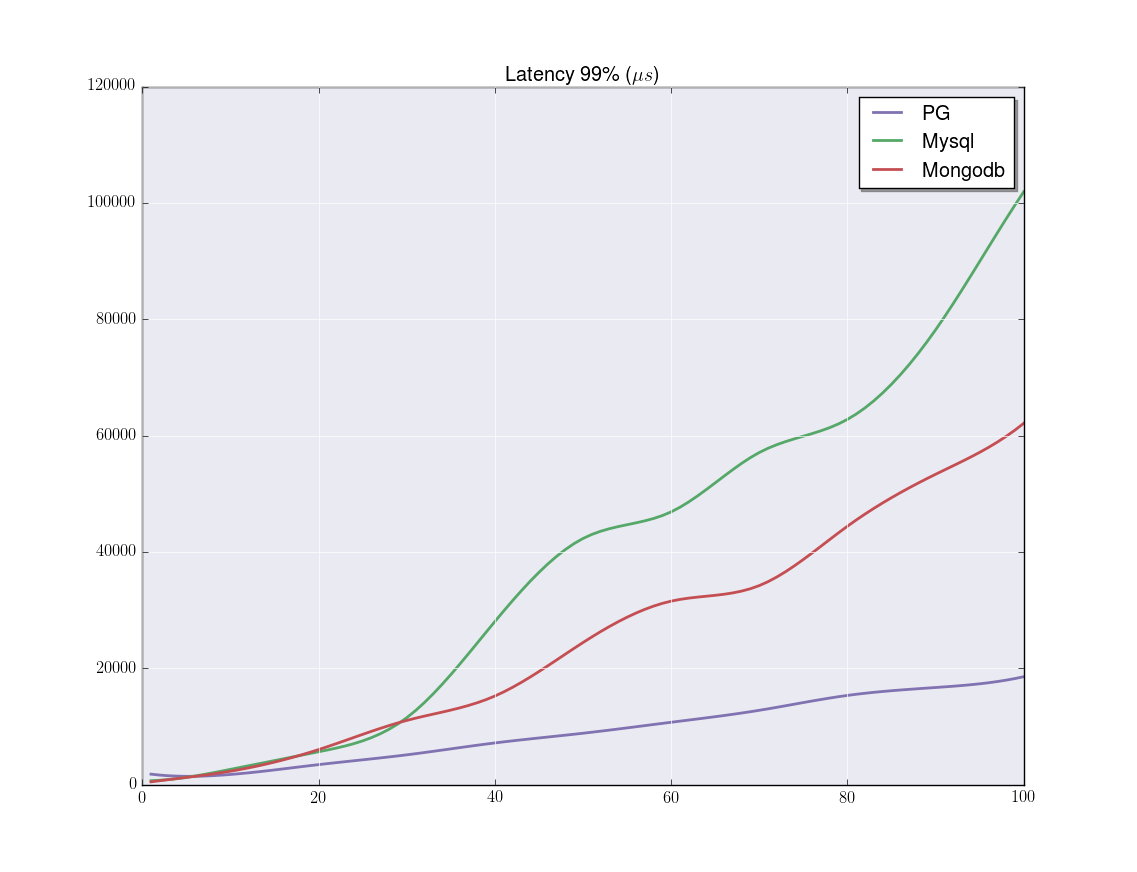
\includegraphics[width=0.75\textwidth,center]{benchmarks/simple_select_latency_99.png}
    \end{figure}
    \end{center}
\end{frame}

%\begin{frame}
    %\frametitle{}
    %\begin{center}
    %\vspace{-10pt}
    %\textbf{Простая выборка по ключу с индексом}
    %\begin{figure}
        %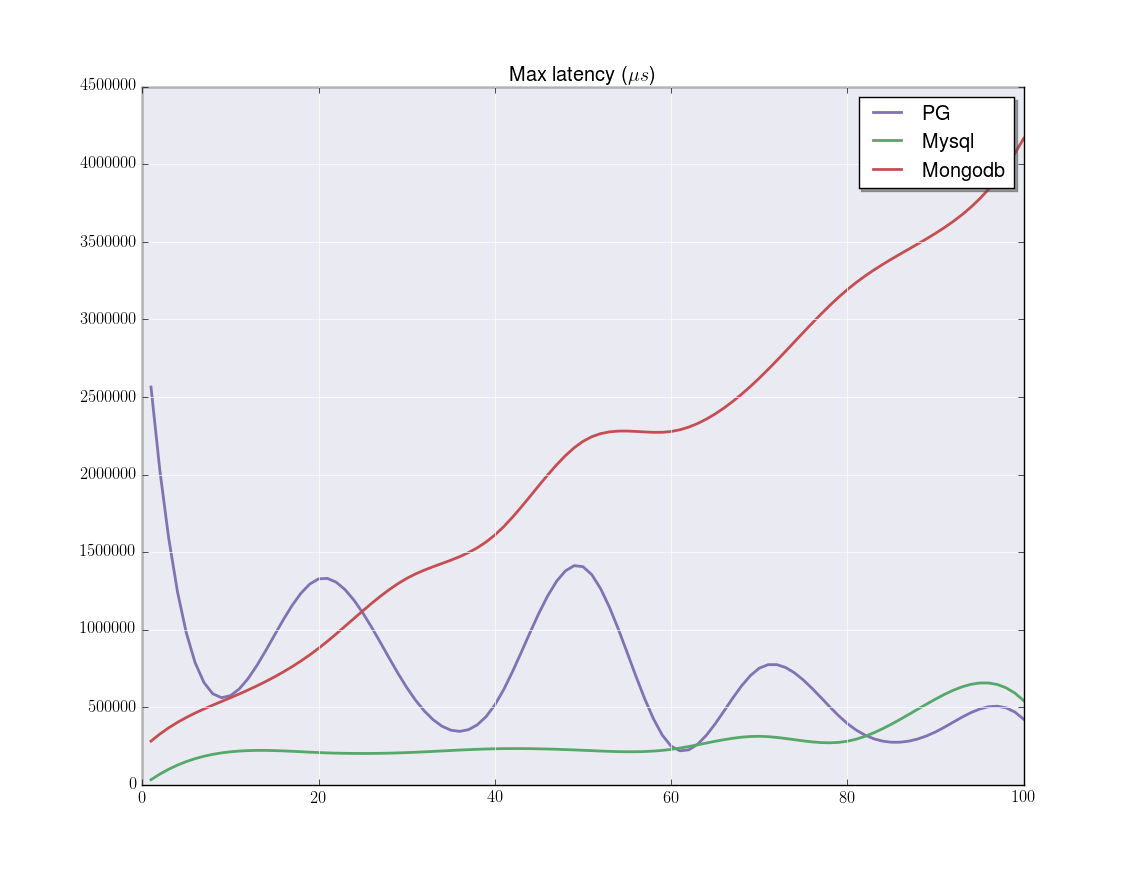
\includegraphics[width=0.7\textwidth,center]{benchmarks/simple_select_max_latency.png}
    %\end{figure}
    %\end{center}
%\end{frame}

\begin{frame}
    \frametitle{}
    \begin{center}
    %\vspace{-10pt}
    \begin{figure}
        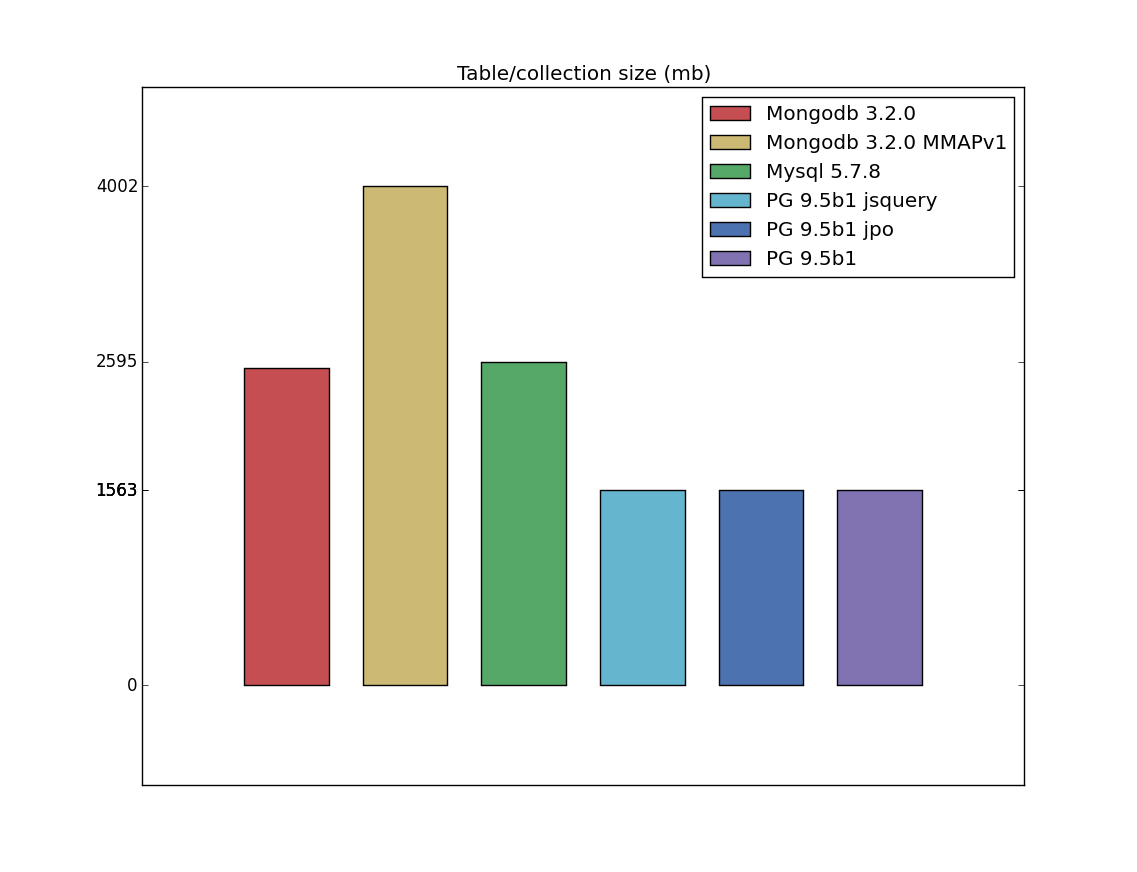
\includegraphics[width=0.75\textwidth,center]{benchmarks/table_size.png}
    \end{figure}
    \end{center}
\end{frame}

%\begin{frame}
    %\frametitle{}
    %\begin{center}
    %\vspace{-10pt}
    %\textbf{Размер индексов}
    %\begin{figure}
        %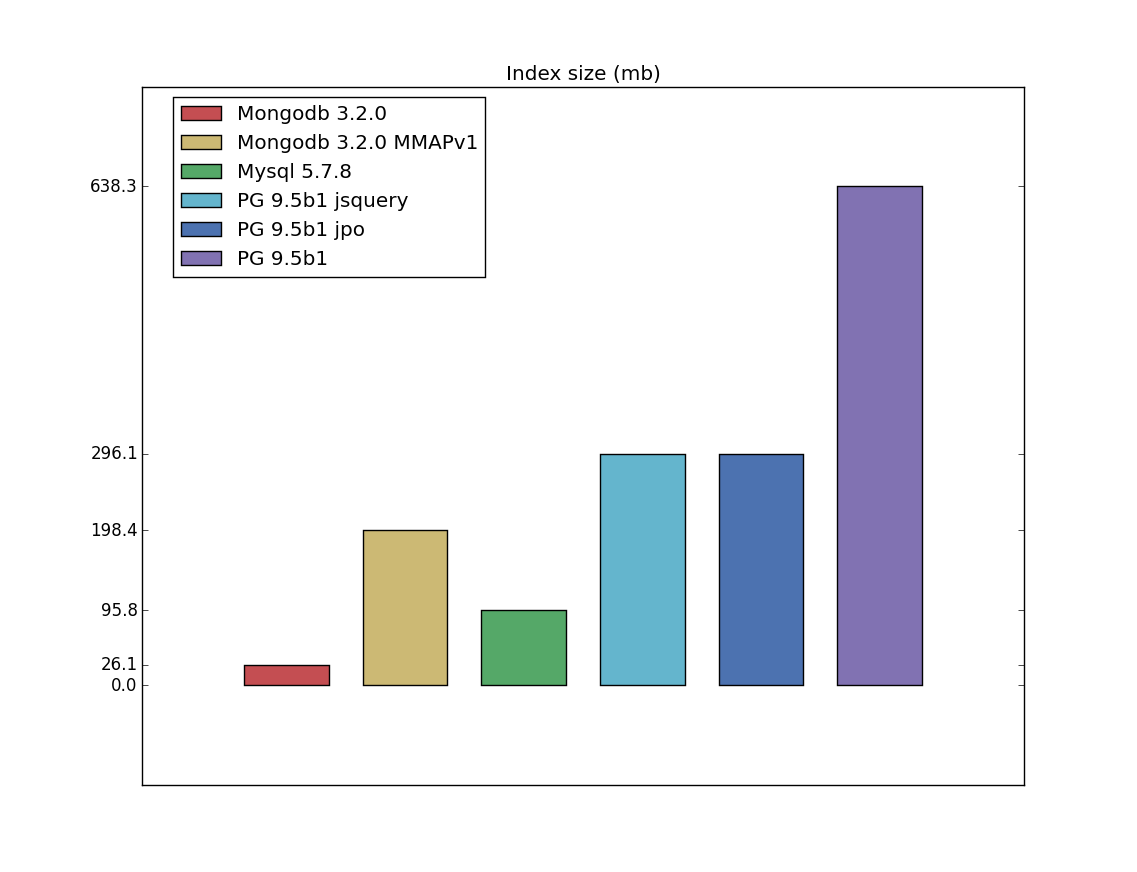
\includegraphics[width=0.7\textwidth,center]{benchmarks/index_size.png}
    %\end{figure}
    %\end{center}
%\end{frame}

\begin{frame}
    \frametitle{}
    \begin{center}
    \vspace{-10pt}
    \textbf{Выборка документов с большим количеством ключей}
    \end{center}
\end{frame}
\note{
    сериализация в ширину
}

\begin{frame}
    \frametitle{}
    \begin{center}
    \vspace{-10pt}
    \textbf{Выборка документов с большой вложенностью}
    \end{center}
\end{frame}
\note{
    сериализация в глубину
}

\begin{frame}
    \frametitle{}
    \begin{center}
    \vspace{-10pt}
    \textbf{Выборка среза по документам}
    \end{center}
\end{frame}
\note{
    множественный detoast
}

\begin{frame}
    \frametitle{}
    \begin{center}
    \vspace{-10pt}
    \textbf{Выборка документов без кэша}
    \end{center}
\end{frame}
\note{
    моделирование ситуации, когда данные не влезают в память
    и идет активная работа с диском
}

\begin{frame}
    \frametitle{}
    \begin{center}
    \vspace{-10pt}
    \textbf{SET STORAGE EXTERNAL}
    \end{center}
\end{frame}
\note{
    хранение jsonb в распакованном формате
}

\begin{frame}
    \frametitle{}
    \begin{center}
    \vspace{-10pt}
    \textbf{Вставка записей}
    \end{center}
\end{frame}

\begin{frame}
    \frametitle{}
    \begin{center}
    \vspace{-10pt}
    \textbf{Вставка и обновление}
    \end{center}
\end{frame}

\begin{frame}
    \frametitle{}
    \begin{center}
    \vspace{-10pt}
    \textbf{Чтение последних}
    \end{center}
\end{frame}

\begin{frame}
    \frametitle{}
    \begin{center}
    \vspace{-10pt}
    \textbf{Чтение, изменение, запись}
    \end{center}
\end{frame}

\fontsize{25pt}{27}\selectfont
\begin{frame}
    \frametitle{}
    \begin{center}
    \textbf{Вопросы?}
    \end{center}
\end{frame}

\end{document}
